\documentclass{article}
\usepackage[utf8]{inputenc}
\usepackage[margin=0.70in]{geometry}
\usepackage{hyperref}
\usepackage{graphicx}
\usepackage{authblk}
\usepackage{subfig}
\usepackage{indentfirst}

\title{Project 4 (Optional): Distillation and Compilation}
\author{Oliver Fowler}
\author{Brian Park}
\affil{North Carolina State University, Computer Science 591/791-025}
\date{November 2022}

\begin{document}
\maketitle
% What to Do 
%
% (i) Go through the Distillation chapter in the User Guide of NNI. 
% (ii) Apply compression (e.g., pruning) to one of the example models in this repository. 
% (iii) After that, apply distillation to improve the accuracy of the pruned model.
% (iv) Install TVM. Go through TVMC tutorial. 
% (v) Apply TVMC to optimize the executions of the model you obtained in (iii). 
% 
% Rubric
% 
% * Overall clarity and completeness of the report: [20]
% * Experiments: [60]
%    compression: 10 points
%    distillation: 20 points
%    TVMC optimizations: 30 points

\section{Distillation and TVMC Optimizations}
% The distillation and TVMC optimizations that you have conducted. 
For the first part of the project, we applied knowledge distillation on a DNN model \cite{distillation}. Distillation requires a compressed model to be trained or distill the knowledge of a pretrained, larger model as shown in Figure \ref{fig:kd-pipe}. We are able to leverage NNI to do compression and then use native PyTorch code to do knowledge distillation \cite{nni, pytorch}. For compression techniques, we are already familiar with pruning and quantization. Unfortunately, NNI's quantization is not well supported, as we have seen from a previous project. So for this project, we only applied pruning.

We also tried additional techniques to speed up training and distillation, such as using mutliple GPUs. Fortunately, bridges-2 nodes have DGX-1 system on \verb|GPU-shared| allocations. An allocation up to 4 V100 GPUs connected via NVLink can be used for data parallel training \cite{v100}. PyTorch natively supports data parallel training on multi GPUs in an intra-node setting via \verb|torch.nn.DataParallel| and \verb|torch.nn.DistributedDataParallel| \cite{pytorch}. We were inspired to use such tasks to fully utilize the supercomputer hardware from related works \cite{imagenet-quick}. Although we successfully trained in a \verb|DataParallel| and \verb|DistributedDataParallel| setting, we realized this process is impossible to apply at the distillation stage. First, NNI creates wrappers around PyTorch modules, making some of the API incompatible with each other. Once a PyTorch model is converted to a distributed setting, it's hard to convert it back to single GPU setting. Plus, we noticed that there is not much work related to distributed distillation on large models to small models, so we moved on to a simpler setup.

\begin{figure}
    \centerline{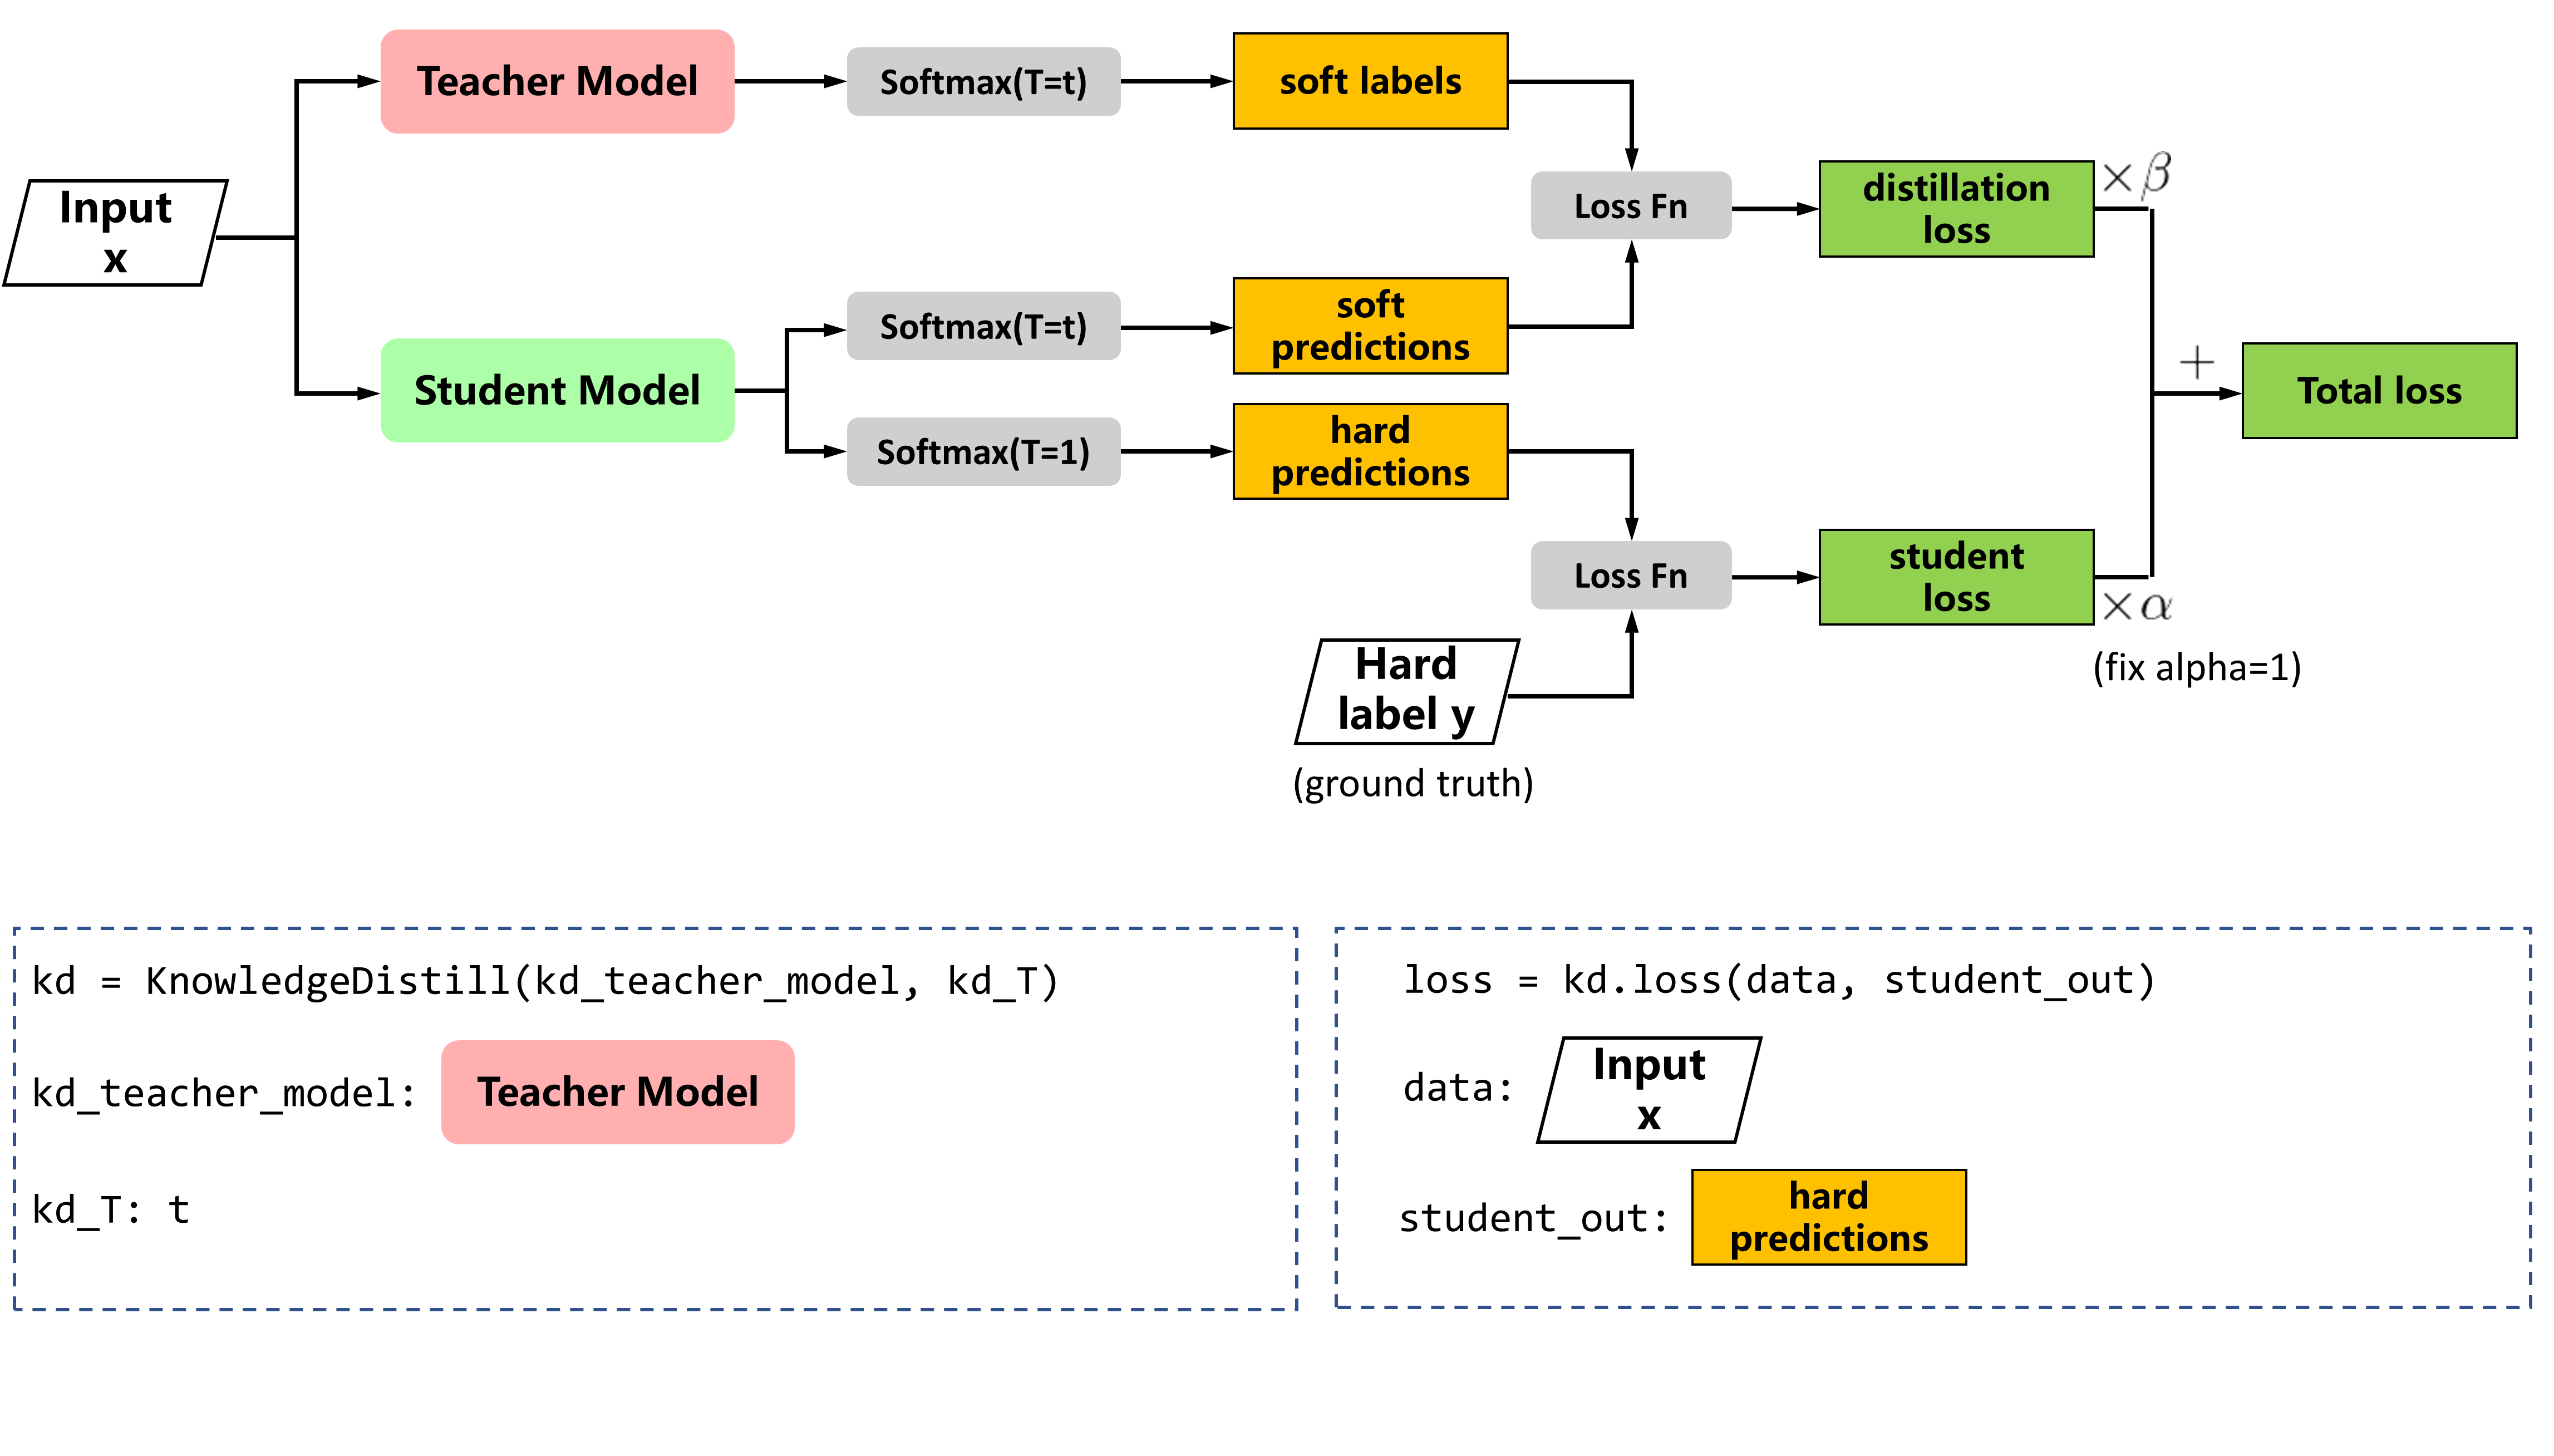
\includegraphics[width=7in]{../proj4/figures/distill.png}}
    \caption{Knowledge Distillation Pipeline \cite{nni}}
    \label{fig:kd-pipe}
\end{figure}

After leveraging NNI and PyTorch to do knowledge distillation to a smaller model, we then used TVM to do end-to-end compiler optimizations to the model \cite{tvm}.
We were able to convert PyTorch to a ONNX file using PyTorch's API. Then we convert the ONNX file to an executable using TVM.

\section{DNN Model}
% The original DNN model, and its forms after (ii), (iii), and (v). 
For this project, we chose ResNet-101 that we previously trained from a previous project on the CIFAR-10 dataset \cite{resnet, cifar10}. Given the time constraint, we didn't want to train a large model from scratch. We actually tried to use DenseNet initially, but ran into issues related to OOM and training speed since we have to load both the teacher and the student model \cite{densenet}. We also tried to skip training from scratch by using the ImageNet dataset, since Torchvision provides pretrained models for it \cite{imagenet, torchvision}. But turns out ImageNet is a very large dataset and it would take days or weeks even on state of the art hardware. We tried some other techniques to utilize the powerful resource of bridges-2 supercomputer, but later realized that NNI and PyTorch makes this process incompatible \cite{bridges-2}.

We chose to distill ResNet-101 model to ResNet-18 model that is also pruned via NNI. We did not apply quantization since NNI doesn't support it properly as we have observed from a previous project. 

The ResNet-18 model is structured pruned via NNI with L1NormPruner with a sparsity of $10\%$ on only \verb|Conv2D| layers \cite{l1prune}. We could not apply pruning on \verb|Linear| layers as the distillation process becomes broken due to incompatible tensor sizes.

\begin{figure}
    \centerline{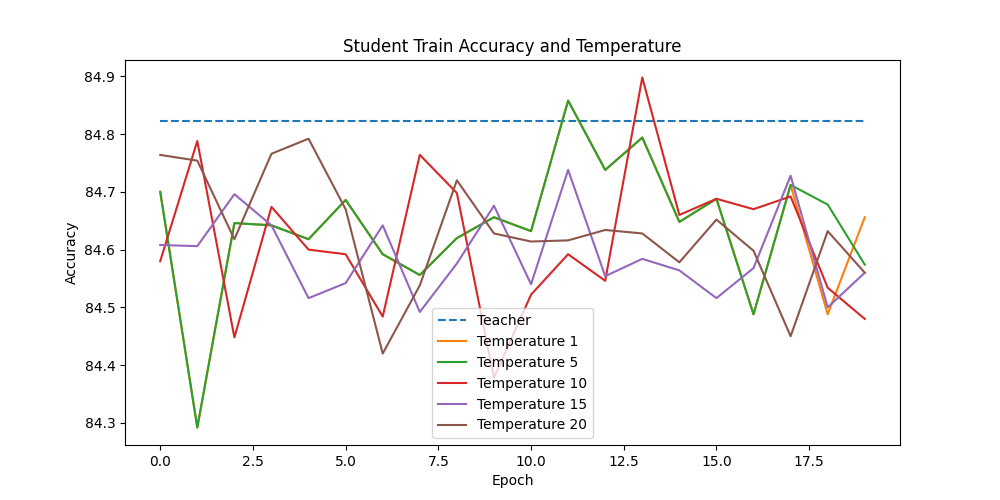
\includegraphics[width=7in]{../proj4/figures/kd_training.png}}
    \caption{Knowledge Distillation Training Accuracy over Epochs}
    \label{fig:kd-training}
\end{figure}

Since there is extra hyperparameter of temperature in knowledge distillation, so we tried temperatures of $T = 1, 5, 10, 15, 20$, just like how Hinton experimented between values of $T$ from 1 to 20 \cite{distillation}. We train and finetune the weights for 20 more epochs. 

After distilling in PyTorch, we converted it to ONNX model files and then to TVM compiled executables. Unfortunately, we couldn't get TVM to compile to a GPU target due to an unknown issue with CUDA libraries not being able to be found and linked properly. Instead, we compiled to LLVM target and benchmarked on the CPU for a fair comparison across optimizations.

For TVM, we also applied tuning that uses XGBoost to automatically tune the performance of the TVM executable \cite{xgboost}.

\section{Experimental Results}
% The accuracy and speed of the original model, and its variants after (ii), (iii), and (v). Explain the reasons for the differences.  
The original ResNet-101 model, or teacher model has a training accuracy of 84.822\% and a validation accuracy of 79.27\%. When applying distillation, we got a training accuracy of 84.6\& on the ResNet-18 distilled model. In the end, we chose the distilled model with a temperature of 1 since it had marginally best training accuracy. Figure \ref{fig:kd-training} shows the training accuracy over epochs. It makes sense that the distilled model should not outperform the teacher model. Unfortunately, changing the temperature doesn't vary a lot, and it's also suspicious why the training accuracy starts off already high. Compared to related works where Stanton experiments and questions the knowledge distillation works, it seems that we may have a flaw in our experimental methodology \cite{distillation-works}.

Figure \ref{fig:tvm-benchmarks} shows the benchmarks of each framework on the CPU of bridges-2, which has a Intel(R) Xeon(R) Gold 6248 CPU. We took one sample image from CIFAR-10. From PyTorch to TVM tuned model, we decreased inference time from 12.97 ms to 8.90 ms for ResNet-101 alone. For ResNet-18 with knowledge distillation the inference time decreased from 5.35 to 2.64. We see that 2-3 ms is saved from just TVM. 

\begin{figure}
    \centerline{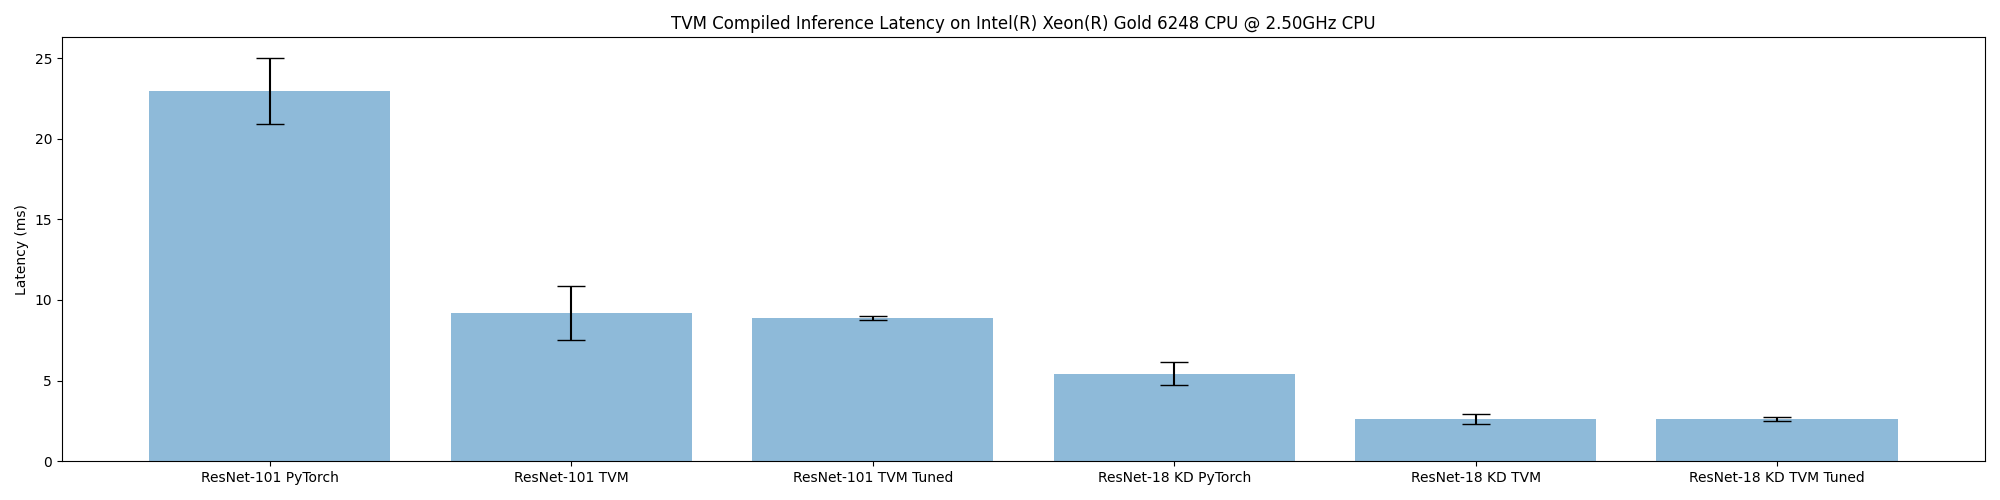
\includegraphics[width=7in]{../proj4/figures/tvm_benchmarks.png}}
    \caption{PyTorch vs TVM Benchmarks}
    \label{fig:tvm-benchmarks}
\end{figure}

The model size doesn't change at all between compilation phases, since we aren't modifying the weights in the compile phase. But interestingly, we see that for ResNet-101 the model size is 170 MB, while the distilled smaller model is 41 MB. At least with knowledge distillation, we're able to retain accuracy within a percent, as well as gain $4.14\times$ size reduction and $4.95\times$ speedup on inference time with compilation optimizations. If this was video processing application where images are streamed, we'd increase processing performance from 77 FPS to 379 FPS.

\section{Lessons Learned}
% What lessons you have learned through the project.
Since we had much powerful compute resources, we took this as a learning opportunity to learn how to utilize it for deep learning. The number one issue we faced is waiting. Since there was only over a week to complete this assignment, we engineered how to make workflow quicker. We subsampled our dataset as well as used multiple GPUs for data parallelism. We can clearly see how deep learning workloads take days or months to train. Fortunately, we made sure to start early.

We also learned how to use TVM. Overall it's very simple to use. If we had more time, we wish we figures out how to properly link CUDA libraries and compile to a GPU target for even more speedup.

Overall, we learned how to do a full stack integration with NNI and TVM for model compression and compilation. We started with a large model and optimized it for a target, which was the V100 GPU in our case. The tools really helped in easing the workflow, as the whole pipeline takes few lines of code and is really simple to program.


\section{GitHub Repository}
% A link to your github repository that contains all the scripts used in this project and a README describing the structure of the repository and how the folders in the repository correspond to the items in the report. The report must be in PDF, with the five required parts clearly marked. 
The GitHub repository for this report is publicly accessible here \cite{proj4-repo}. To reproduce our findings, please read the \verb|README.md| under the \verb|proj4| directory. If there are any setup issues on bridges-2 supercomputer or locally, please contact \href{mailto:bcpark@ncsu.edu}{bcpark@ncsu.edu}.

\bibliographystyle{ieeetr}
\bibliography{references}


\end{document}